\documentclass[11pt,twocolumn,letterpaper]{article}

\usepackage{cvpr}
\usepackage{times}
\usepackage{epsfig}
\usepackage{graphicx}
\usepackage{amsmath}
\usepackage{amssymb}
\usepackage[breaklinks=true,bookmarks=false]{hyperref}
\usepackage{color}
\usepackage{indentfirst}
\usepackage{listings}
\definecolor{codegreen}{rgb}{0,0.6,0}
\definecolor{codegray}{rgb}{0.5,0.5,0.5}
\definecolor{codepurple}{rgb}{0.58,0,0.82}
\definecolor{backcolour}{rgb}{0.95,0.95,0.92}


\lstdefinestyle{mystyle}{
  backgroundcolor=\color{backcolour},
  commentstyle=\color{codegreen},
  keywordstyle=\color{magenta},
  numberstyle=\tiny\color{codegray},
  stringstyle=\color{codepurple},
  basicstyle=\footnotesize,
  breakatwhitespace=false,
  breaklines=true,
  captionpos=b,
  keepspaces=true,
  numbers=left,
  numbersep=5pt,
  showspaces=false,
  showstringspaces=false,
  showtabs=false,
  tabsize=2
}
\lstset{style=mystyle}
\cvprfinalcopy % *** Uncomment this line for the final submission

\def\cvprPaperID{****} % *** Enter the CVPR Paper ID here
\def\httilde{\mbox{\tt\raisebox{-.5ex}{\symbol{126}}}}

% Pages are numbered in submission mode, and unnumbered in camera-ready
%\ifcvprfinal\pagestyle{empty}\fi
\setcounter{page}{1}
\begin{document}

%%%%%%%%% TITLE
\title{
Computer Vision Course Project Report\\
Gambody
}

\author{Rong Yuyang, Cai Jianxion, Li Ziyue, Huang Jingyi, Pang Anqi\\
School of Information Science and Technolody\\
ShanghaiTech University\\
{\tt\small \{rongyy, caijx, lizy, huangjy, pangaq\}@shanghaitech.edu.cn}
}

\maketitle
%TODO add github link maybe, note that the version with body region tracking is not v2.0 (master), it is on the branch v2.2.
\begin{abstract}
  In this report we propose our implementation of a game where the user have to do certain pose to pass and only a camera on laptop is required. 
  In this report we will explain out methods and the iteration of this game. 
  We started off by simply subtracting the image stream with the background, and we ended up with Openpose and noise cancellation.
  In the end we implemented an interesting game with noise cancellation and accurate check rate.
\end{abstract}
\section{Introduction}
    \par We found a popular game called \textit{Hole in the Wall}. In this game one (or two) player(s) are facing a moving wall with a certain shape of hole, the player have to make a specific pose to pass the moving wall or he will be pushed into a water pool behind him. Such a game is interesting but householders can never have the privilege to play in family gatherings or parties since one can hardly find a moving wall nor adequate safety measurements.
        \begin{figure}[h]
            \centering
            
\includegraphics[width=0.8\linewidth]{./Pic/HIW_Logo}
            \caption{Game Logo}
        \end{figure}
        \begin{figure}[h]
            \centering
            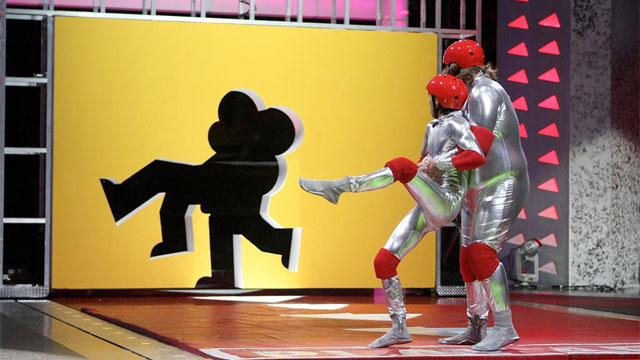
\includegraphics[width=0.45\linewidth]{./Pic/HIW_RedTeam}
            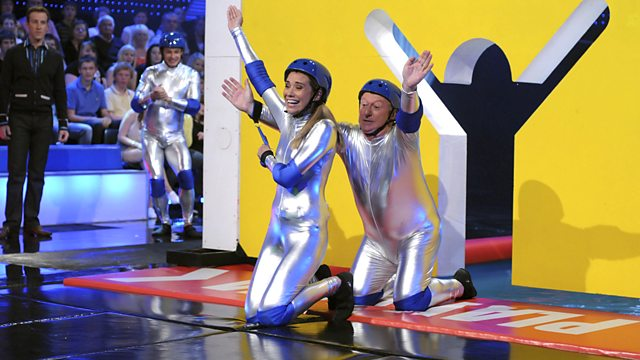
\includegraphics[width=0.45\linewidth]{./Pic/HIW_BlueTeam}
            \caption{Two players in the game posing to pass the wall.}
        \end{figure}
    \par To fix this, we are going to implement a system based on camera so that every one can play this game.
        In our work, we will be using one single camera to track person. It will also give player a bounding box (moving wall), which is remarked as a mask in the system.
        The mask and player's body part is compared by our system, the return should be a pass (True) or no pass (False). More details about our technical approaches are in Section 3. And the subsection Mask Generation introduces how to generate masks.
    \par In Section 3, we will propose two versions of implementations. In the first version, we apply direct subtraction to get the body part of the player and return a pass if the overlap of body and mask is greater than a threshold. More details are included in the subsection Version One. Since this naive version is parameter-dependent and has low robustness, we implement a more advanced version based on a previous work \textit{Realtime Multi-Person 2D Pose Estimation using Part Affinity Fields}\cite{cao2017realtime}. Specifically, we compare the skeletons of the mask and the player and define a loss function computing the euclidean distance. Likewise, the system returns a pass if the loss is smaller than a threshold. More details about this version are included in the subsection Openpose.
    \par In both versions, we have no need to care about object noise. But there may be circumstances where some unexpected passers-by appear resulting in the ambiguity of deciding which is the player. To deal with this kind of noise, we have tried out two solutions. One is called \emph{highest wins} strategy, and the other bases on \emph{trajectory predition}. The efforts on noise cancellation are presented in the subsection Noise.
    \par We also did some experiments to improve the system further. In Section 4, the trials about \emph{weights on skeleton} and \emph{noise cancellation parameters} are introduced in detail respectively.
\section{Related Work}
Our goal is to get 2D or 3D stable skeleton from single webcam with out depth channel(using only RGB) in real time. We focus the discussion of related work on approaches of using other camera and not in real time. We will also introduce some real-time skeleton reconstruction with one single camera.
  \subsection{Multi View}
  With multi-view setups markerless motion-capture solutions attain high accuracy, and it is also easy to get the depth information from multi-view.Most methods target high quality with offline computation \cite{Loper2014}\cite{twist}.Robustness could be increased with a combination of generative and discriminative estimation \cite{7299005}, even from a single input view \cite{Rosales2006}.
  \subsection{Monocular Depth}
  The depth channel provided by RGB-D sensors has led to robust real-time pose estimation solutions\cite{6126356}\cite{7457693}. Even real-time tracking of templete free reconstruction is now available\cite{Dou:2016:FRP:2897824.2925969}.The depth information overcome forward-backward  ambiguities in monocular camera. Our goal is to use one webcam to achieve 2D or 3D skeleton reconstruct.
  \subsection{Monocular RGB}
  These approach is what we need, one is the real-time  full global 3D skeletal pose of a human in a stable, temporally consistent manner using a single RGB camera method \cite{VNect_SIGGRAPH2017}, but it cost much resource especially when we want to build a game on a poor platform.\\
  Another is the openpose method\cite{cao2017realtime}\cite{wei2016cpm}, they efficiently detect the 2D pose of multiple people in an image. The approach uses a nonparametric representation to learn to associate body parts with individuals in the image. This is also the method we use.
  \subsection{Body Region Tracking}
  Recently, lots of research has been developed on body (object) tracking including features-based tracking, counter-based tracking \cite{panin2006efficient} and region-based tracking \cite{1640835}.
  \par
  In region-based tracking, lots of different approaches have been developed for tracking non-rigid object. The shape human body, unlike that of rigid objects, will change with body movement.
  \par
  In 2006, A. Adam and E. Rivlin and I. Shimshoni proposed a robust approach with fragments-based tracking. In 2014, Kwon proposed double bounding box approach to handle ambiguous regions. \cite{Kwon2014}

\section{Technical Approach}
	\subsection{Mask Generation}
		\par We generate mask by taking a photo of a pose and the background first.
		Then we subtract the image to get the binary mask of the pose.
		We also use Openpose to generate a skeleton data and image.
		\begin{figure}[h]
			\centering
			
\includegraphics[width=0.45\linewidth]{./Pic/Approach_Mask_back}
			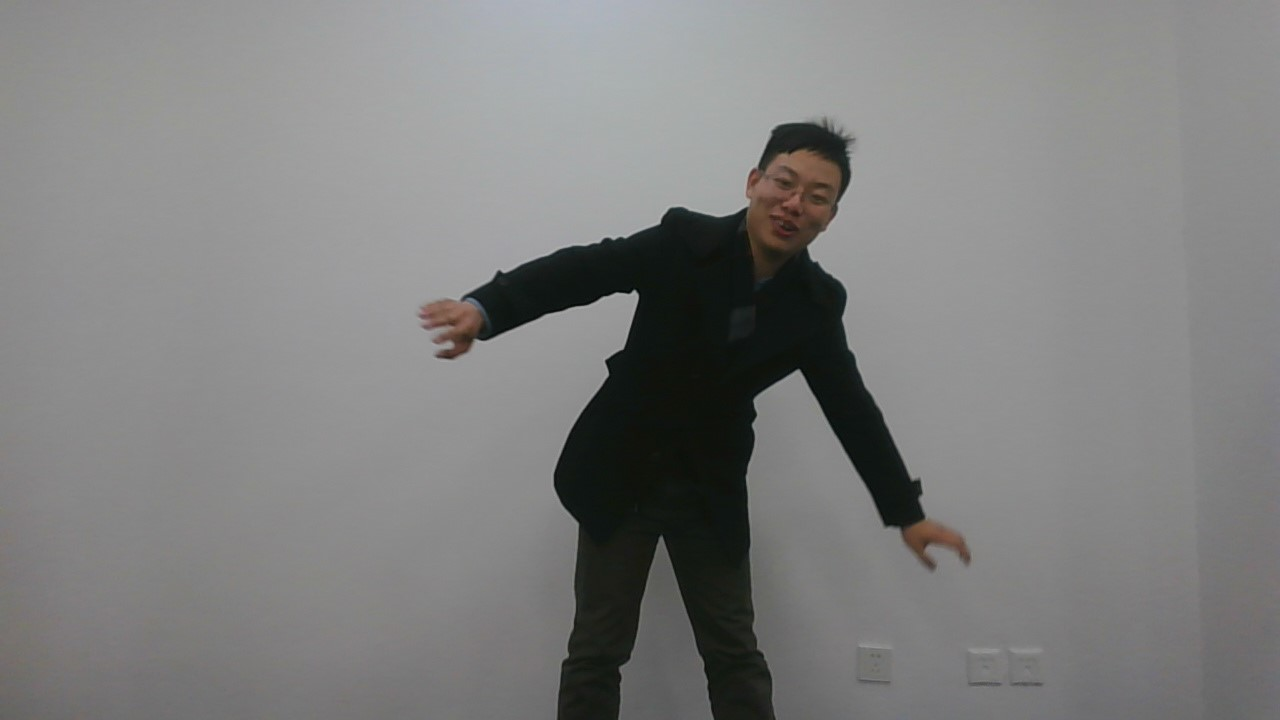
\includegraphics[width=0.45\linewidth]{./Pic/Approach_Mask_pose}
			\caption{Initial images given}
		\end{figure}
		\begin{figure}[h]
			\centering
			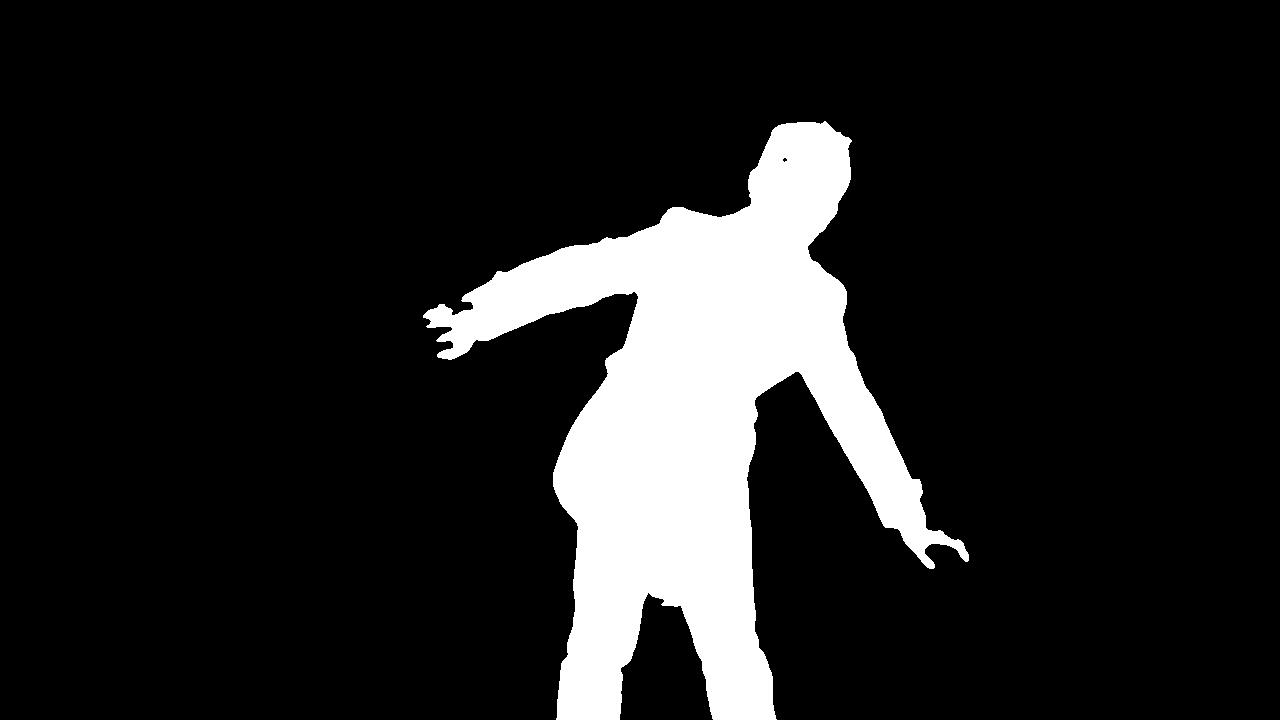
\includegraphics[width=0.9\linewidth]{./Pic/Approach_Mask_binary_mask}
			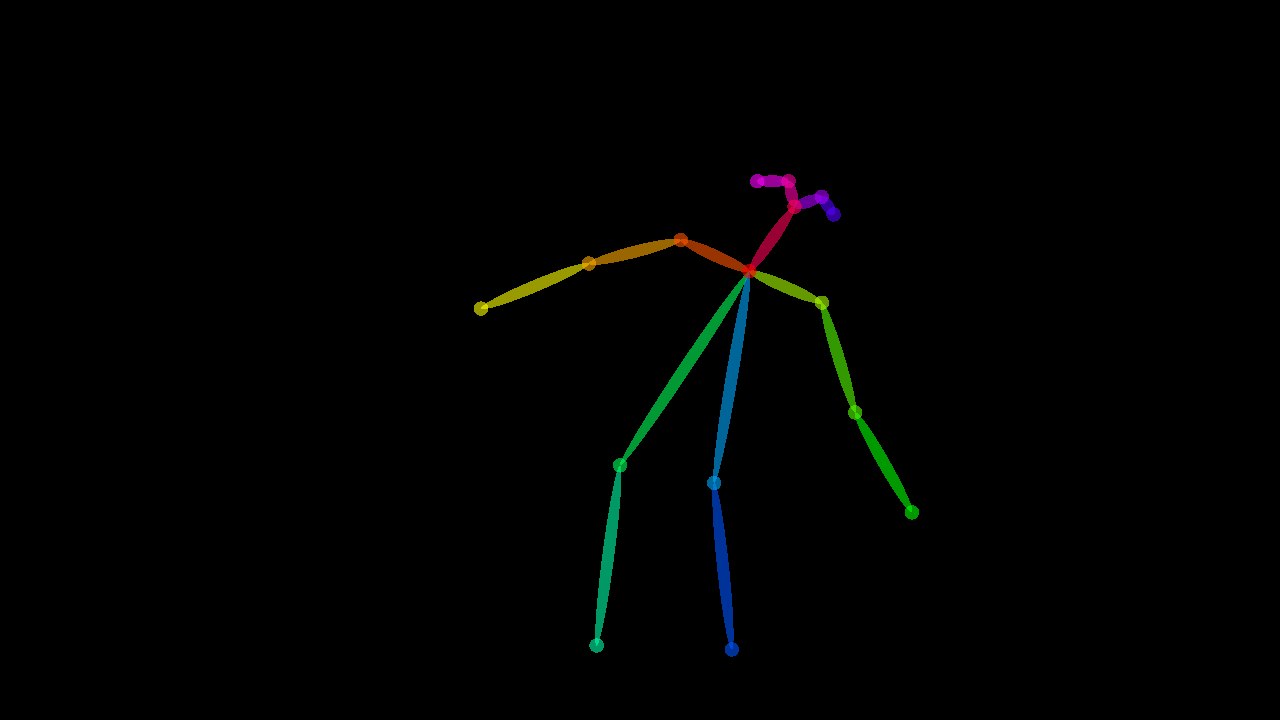
\includegraphics[width=0.9\linewidth]{./Pic/Approach_Mask_skeleton}
			\caption{Mask generated}
		\end{figure}
	\subsection{Version One}
        \par We implemented a first version of system in the early stage of this project. To achieve real-time image processing and displaying, we keep on capturing an image from the camera stream, modifying the image, and showing it on the screen. An infinite loop is kept so. For image processing, the pipeline is shown in Figure 5.
        \par Based on the fact that the background doesn't change during the game time, we capture a background image at the very beginning. Subtracting it from the image having the player, the body part is obtained roughly, which is just the remainder.
        \par However, the subtraction result may have some noise, especially the edges because of the unavoidable camera shake. To eliminate the edge effects, we use a gaussian filter to blur the images before doing subtraction.
        \par Another problem remained is that the body detected may be isolated, particularly the head. So we have to find the two maximum connected components and combine them together to get the complete body part.
        \par Finally, provided with the mask image and the body image, we compare them by computing the normalized correlation ratio. If the maximum value (the best match ratio) is greater than a pre-set threshold, the system returns a pass to the player.
        \begin{figure}[htbp]
			\centering
			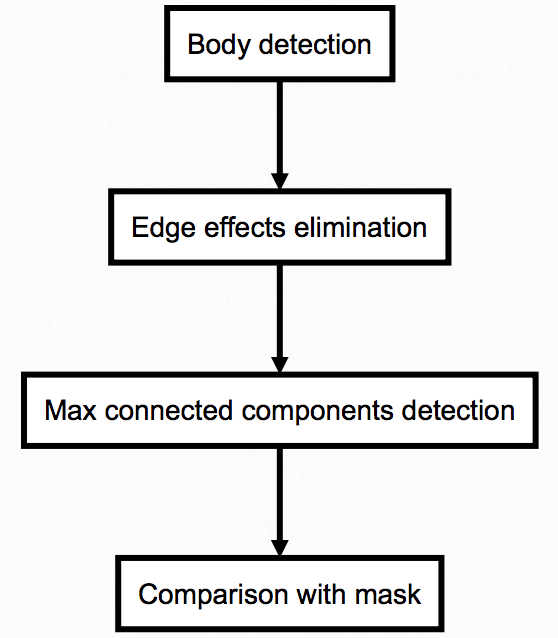
\includegraphics[width=0.9\linewidth]{./Pic/flowchart.png}
			\caption{Pipeline for image processing in Version One.}
		\end{figure}
		\par
		After finishing version 1, because the following reason, we start to implement several crucial improvements in later versions, which is introduced following.
		\begin{itemize}
		\item The cropped body is greatly affected by noise in the background (like moving object).
		\item Camera shaking and ambiguity with body and background have great impact on the final result.
		\end{itemize}
	\subsection{Openpose\cite{cao2017realtime}}
	    \par To generate a skeleton we have to generate confidence map using which we can determine where the joint is.
		Each joint is self-defined, so joint here can be eyes and ears.
		18 joints is defined, which is eyes(2), ears(2), nose(1), chest(1), shoulders(2), elbows(2), wrists(2), waists(2), knees(2) and ankles(2).
		We also have to predict Part Affine Fields, which can be used to generate a cost for each connection.
		\par With joints and connection cost, how to connect joints become a bipartite graph maximum matching problem.
		\par We used the binary executable\cite{cao2017realtime} when testing. We will take the last image and give it to the executable. The executable will generate a json file describing each detected joint for each person.
	    \subsubsection{Json}
        \par As the skeleton information returned from openpose is json, we need to extract information from it and use in Matlab. So we use a built string manipulation library for json. The license is in $jsonlab$ folder.
        \par After getting the structure returned, we can check the workspace and withdraw the skeleton information. Skeleton data stored form is cell in matlab, we use the $jsonlab$ for each skeleton and convert data from cell to matrix once for all so as to running faster and handle easily.

	\subsection{Noise}
\par
So far, background noise is no going to affect openpose, as they will not be regarded as human bodies. However, if another person is presented in front of the camera, like if a person happen to pass by. (As is shown in fig. \ref{tracking} ) It could bring confusion to the final judgment because the Openpose will detect two different person. We implemented two different approaches to slove that problem.
\subsubsection {Naive approach with assumption}
\par
First, given the assumption that the user is more close to the target than other people, we can simply calculate scores for every body pose and take the highest one as the player's score.
\par
However, we realized that if someone is intentionally testing the system, it does not make sense if we can't identify player and other people. As the result, we are using a simplified body region tracking approach.
\subsubsection{Body region tracking}
      \begin{figure}[h]
      \centering
      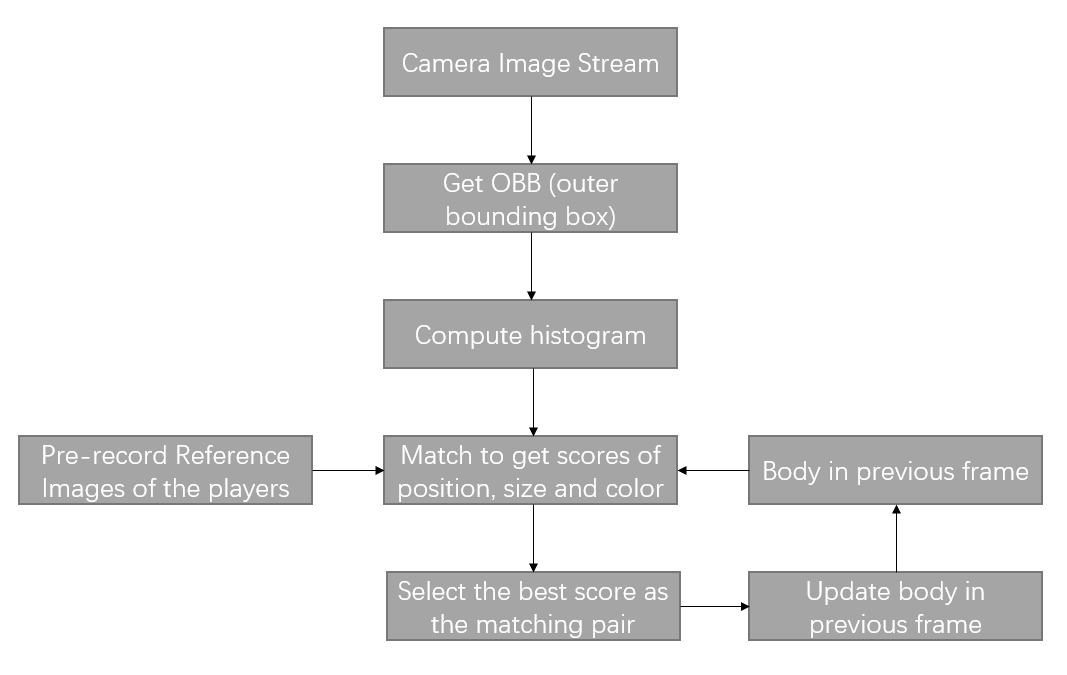
\includegraphics[width=\linewidth]{./Pic/tracking-pipeline.png}
      \caption{The pipeline for the tracking part}
      \end{figure}
\par
Our approach is similiar to the approach in fragments-based tracking  \cite{1640835}. We made serveral sacrifices due to real-time performance. Because  we are using MATLAB, so we need a really simple and fast approach. 
\par
\subsubsection*{Assumptions}
\begin{itemize}
\item The player is always in front of the camera.
\item The camera frame rate is high enough so that the player's shape and location will change continously and slightly each frame.
\item The player has pre-recorded images or he can submit those image in the initialization stage of the game.
\end{itemize}
\subsubsection*{Body Patch Representation}
\par
Our approach is using the outter bounding box (OBB) to represent the body patch. We regard the whole bounding box as one large patch and does not split it up for real-time performance.
\subsubsection*{Define features}
      \begin{figure}[h]
      \centering
      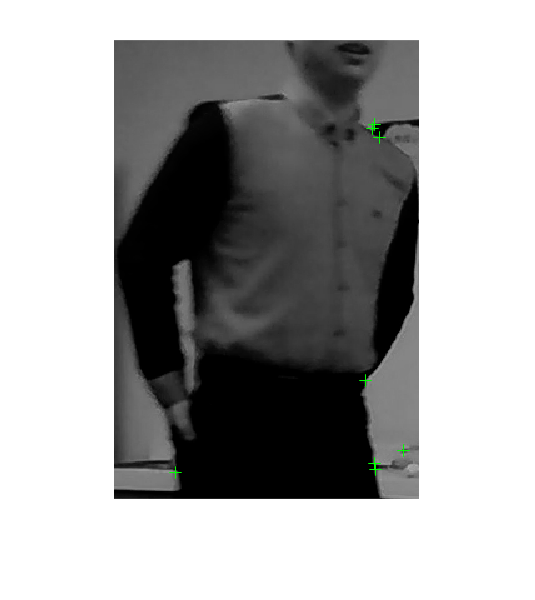
\includegraphics[width=0.45\linewidth]{./Pic/FAST.png}
	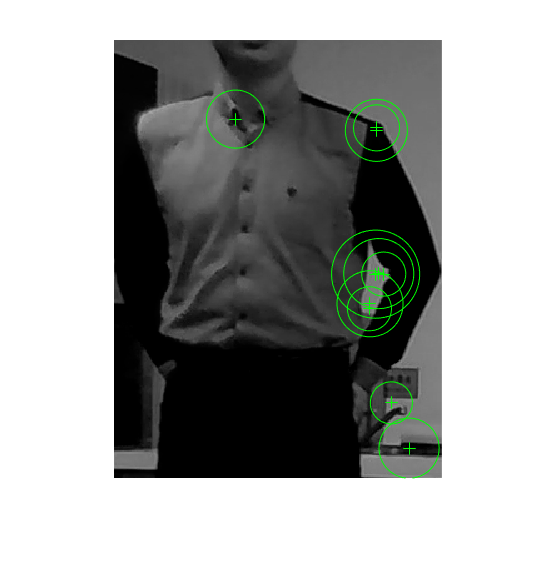
\includegraphics[width=0.45\linewidth]{./Pic/SURF.png}
      \caption{FAST corner extarction (left) and SURF descriptors (right). Only a little unstable features are extarcted.}
      \end{figure}
We are using three low-level featuers to track the player: position on 2D image plane, size of the bounding box, and the color histogram. The main reason is that features extraction and descriptors, like FAST \cite{1544896} and SURF \cite{Bay2006}, have poor performance on textureless clothes, occulusion, and non-rigid objects.
\subsubsection*{Define scores}
There is a various ways on define the score functions for each feature, the general priciple is that 
\begin{itemize}
\item The smaller the position change of the player between adjacent frame, the similiar those two patches are.
\item The smaller the size of OBB changes, the similiar those two patches are.
\item For color histogram, simply calculate the coresponsing bins would be enough. Of course, it is possible to change to other distance measurements.
\end{itemize}
\par
In the end, all three scores are weighted sum up to give a total score for each possible matching pair. Detail score defination will be shown in the experiment section.
\subsubsection*{Robustness}
\begin{figure}[h]
      \centering
      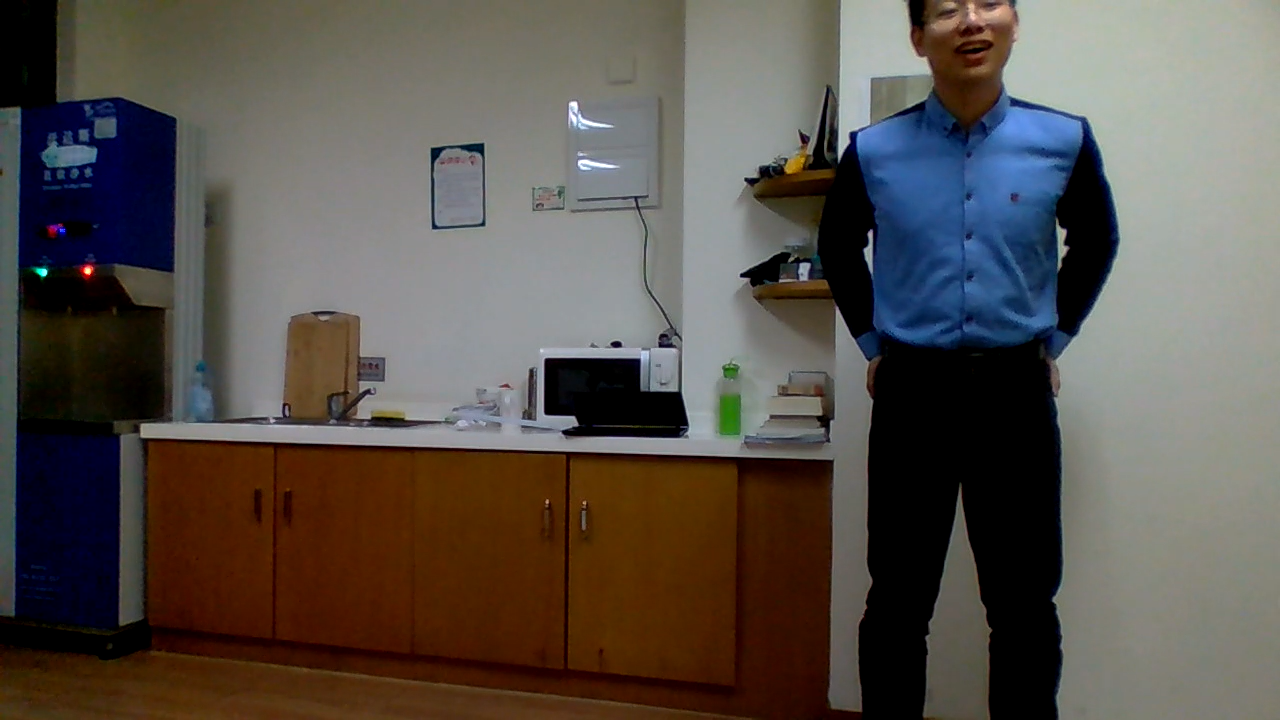
\includegraphics[width=0.45\linewidth]{./Pic/ref-1}
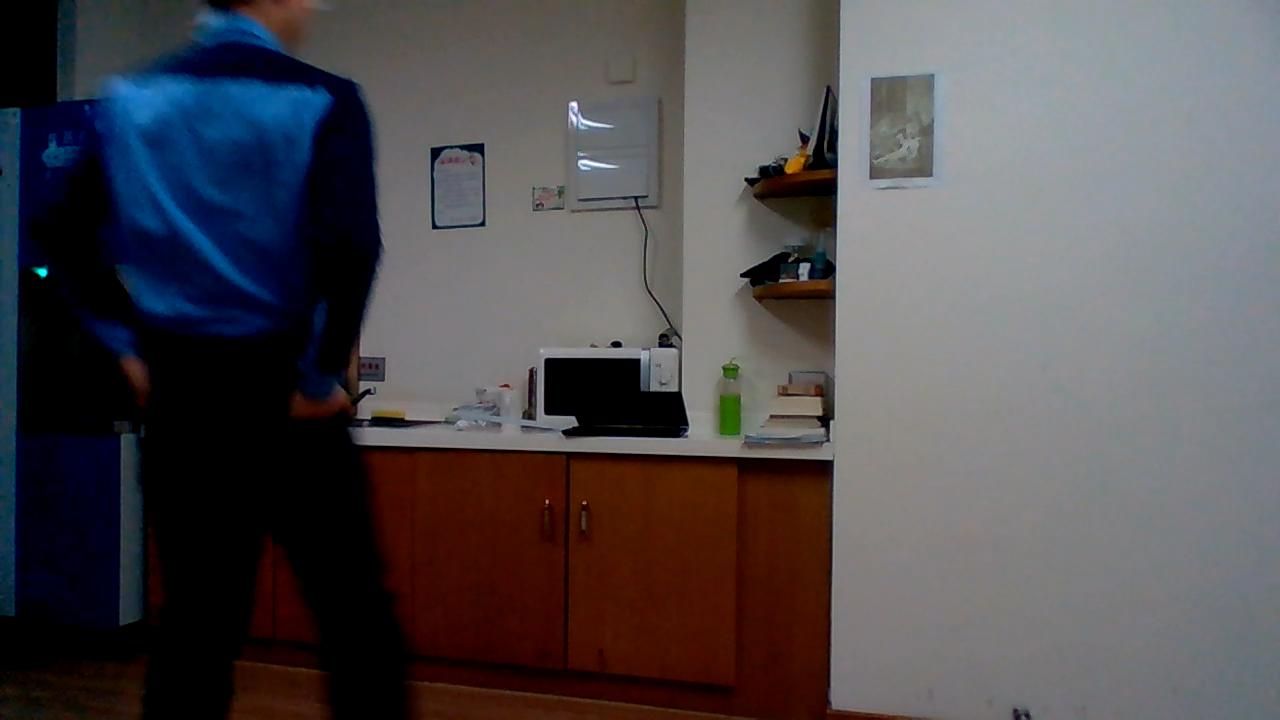
\includegraphics[width=0.45\linewidth]{./Pic/ref-2}
      \caption{Pre-record reference images of player with different pose before tracking start}
      \end{figure}

Because we use OBB as one big patch, this sacrifice rubustness for real-time performance. The system could loss tracking when player turn around, so the player is required to submit or capture images of different poses (reference images) before the game. All current frame are matched with those reference images and the previous frame. This gives us two benefits:
\begin{itemize}
\item If the player turn around, the system can keep tracking with the reference image of a different pose.
\item Even if we loss tracking, the system can recover tracking if the current frame is similiar enough to the reference frame.
\end{itemize}
\section{Experiment}
	\subsection{Weight on Skeleton}
      \begin{figure}[h]
      \centering
      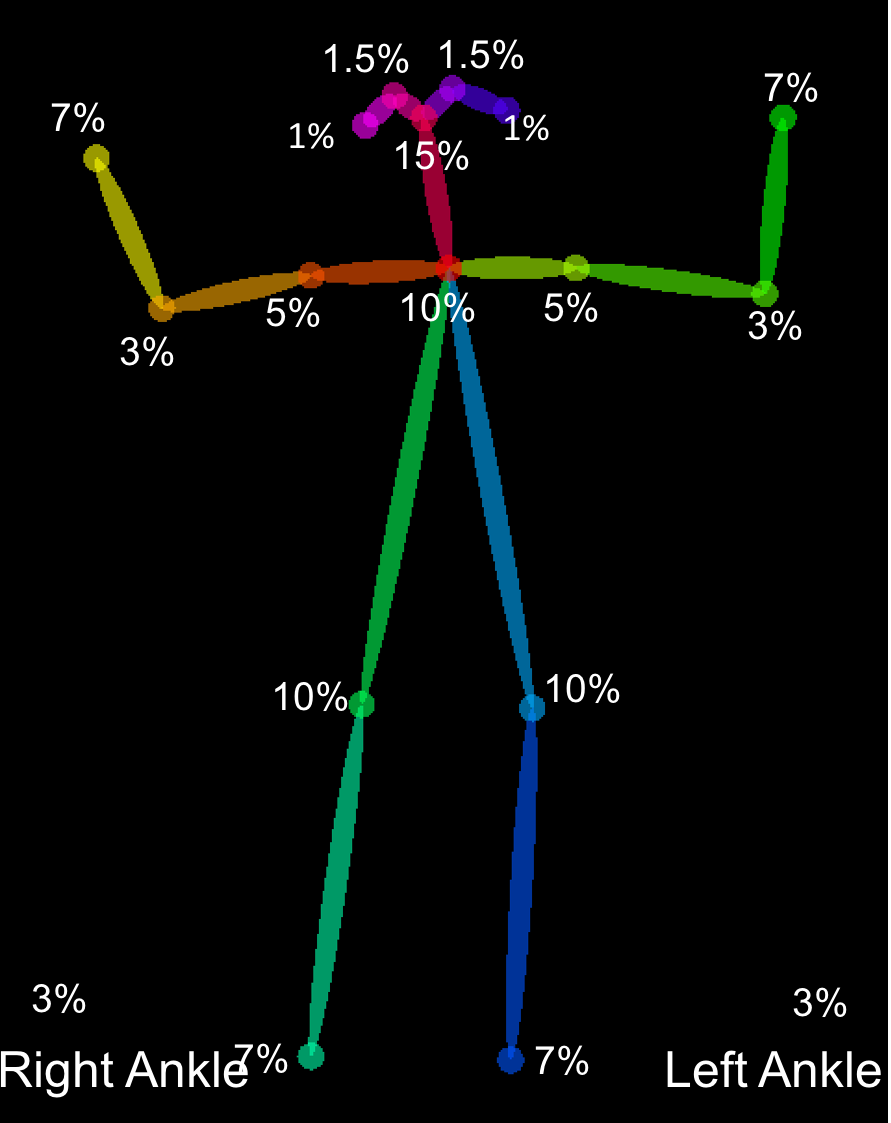
\includegraphics[width=0.8\linewidth]{./Pic/skeleton}
      \caption{Weight on Skeleton}
      \end{figure}

      \par In order to compare the closeness degree between the skeletons of player and mask provided, our initial idea is to add up euclidean distances of corresponding points if their reliability both higher than threshold value we set. We consider the sum as $loss$. So if $loss$ is bigger than threshold value or the total number of reliable correspondence is less than expected, we will determine the player to lose the match. The naive judgment works well in practice.
      \par To improve the judgment based on our ideas such as the pose of trunk should important than limbs, we intend to assign different weight to keypoints in skeleton. Then the influence of each parts unmatched is different. But in experiment, this method doesn't preform better than the naive implementation. In the end, our implementation is still using the naive version.
  \subsection{Body Region Tracking}
\subsubsection{Score function used in real scene}
The score function are defined as an equal combination of position score, size score and color histogram score.
\par
position score: (dist is the body position (pixel) change between current frame and previous frame.)
\begin{equation}
    P_{t}=
   \begin{cases}
   100 &\mbox{if $dist < 300$}\\
   0.8*(400-dist) &\mbox{if $300 < dist < 400$}\\
0.5*(400-dist) &\mbox{if $400 < dist < 500$}\\
0.3*(400-dist) &\mbox{if $500 < dist < 600$}\\
0 &\mbox{if $dist > 600$}
   \end{cases}
  \end{equation}

size score: (A is the OBB of current frame, B is OBB of previous frame, w is with, h is height)
\begin{equation}
    S_{t}=
   \begin{cases}
   100 &\mbox{if $\frac{3}{4} < \frac{A.h}{B.h} < \frac{5}{4} $ \&\& $\frac{1}{3} < \frac{A.w}{B.w} < \frac{7}{4} $}\\
25 &\mbox{Otherwise}
   \end{cases}
  \end{equation}

\par
color score is simply the number of there coresponsing bins.

\subsubsection{Tracking Result}
\begin{figure}[h]
      \centering
      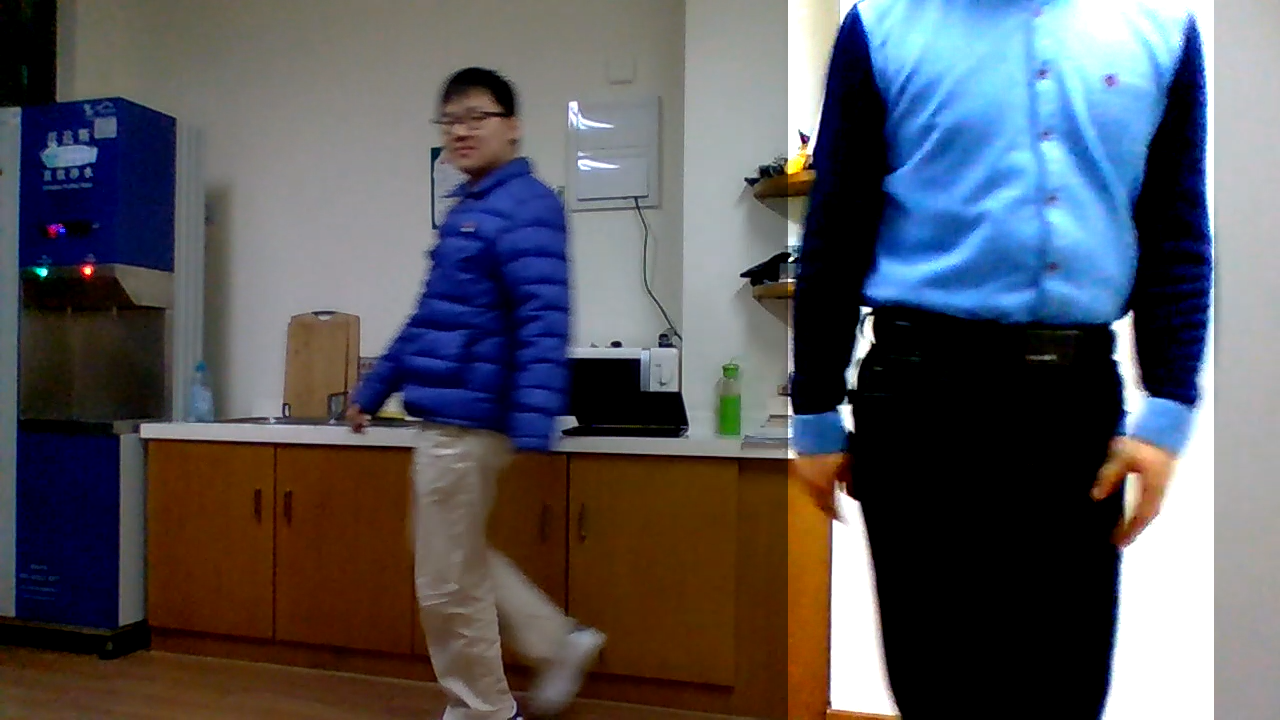
\includegraphics[width=0.8\linewidth]{./Pic/tracking-351.png}
      \caption{Tracking Reult (Frame 351). Player in blue is highlighted with an outter bounding box, and passby person will not be identified as player.}
	\label{tracking}      
\end{figure}
\subsubsection{Real Time}
\begin{figure}[h]
      \centering
      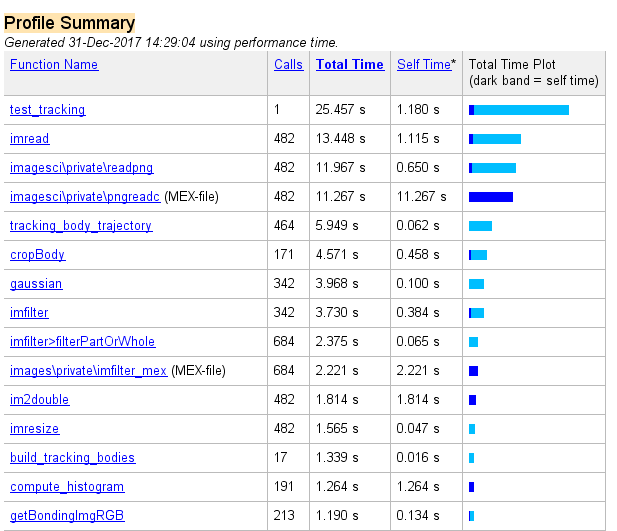
\includegraphics[width=0.8\linewidth]{./Pic/time.png}
      \caption{offline MATLAB time profiling result on a 16-second vedio, containing 464 frames in total. The total time used is 25.457s, where half of the time is used for IO operation.}
\label{timing}      
\end{figure}
 The result is shown in fig. \ref{timing}.  In real application, IO operation time can be avoid as the image stream will not go through the disk. As the result, in real application, the second assumption about frame rate can be achieved even with MATLAB.
\section{Conclusion}
    \par A realtime single RGB-camera based somatosensory game has been produced in our project. We have implemented it from a simple way to a more technical way. Primary related computer vision topics we have put into practice include filtering, pose detection, key point detection, color histogram, tracking and so on.
    \par Honestly, we have learned so much from this project. Studying previous related works broadened our horizons and expanded our minds. Converting theoretical knowledged learned from class into practical work also consolidated our knowledge and improved our programming skills.
    \par Of course there are still some remaining problems to which we have not figured out best solutions, such as a better comparison strategy or noise cancellation scheme. And what's more, we'd better design a more user-friendly UI. Harder masks should be created as well in order to increase the difficulty of the game and make it more interesting. All in all, a lot of improvements can be made if we want to create a real game with high playability.

{\small
\bibliographystyle{ieee}
\bibliography{report}
}
\end{document}
